\documentclass{article}
\usepackage[utf8]{inputenc}
\usepackage[T1]{fontenc}
\usepackage{ngerman}
\usepackage{amsmath}
\usepackage{amsfonts}
\usepackage{a4wide}
\usepackage{color}
\usepackage{colortbl}
\usepackage{graphicx}
\usepackage{url}
\definecolor{rose}{rgb}{1, 0.57, 0.69}		      
		      
\title{Praktikum Multicore-Programmierung \\ Abschlussprojekt 1}
\author{Gruppe 3: Sarah Lutteropp und Johannes Sailer}

\date{\today}
% Hinweis: \title{um was auch immer es geht}, \author{wer es auch immer 
% geschrieben hat} und  \date{wann auch immer das war} k\"onnen vor 
% oder nach dem  Kommando \begin{document} stehen 
% Aber der \maketitle Befehl mu\ss{} nach dem \begin{document} Kommando stehen! 
\begin{document}

\maketitle


\begin{abstract}
Dies ist eine Ausarbeitung für das Abschlussprojekt des Praktikums Multicore-Programmierung im Wintersemester 2015/16. Ziel des Projektes war es, am Beispiel des Jacobi-Verfahrens und des Gauß-Seidel-Verfahrens parallele Lösungsmethoden partieller Differentialgleichungen zu implementieren. Wir haben sowohl das Jacobi-Verfahren als auch das Gauß-Seidel-Verfahren mittels OpenMP parallelisiert. Hierbei haben wir für das Gauß-Seidel-Verfahren sowohl einen Parallelisierungsansatz mittels Wavefront als auch einen Parallelisierungsansatz mittels Rot-Schwarz-Unterteilung gewählt. Unsere mit SIMD-Instruktionen beschleunigte Rot-Schwarz-Implementierung des Gauß-Seidel-Verfahrens zeigte die schnellste Laufzeit bei unseren Messungen, gefolgt von der nicht vektorisierten Rot-Schwarz-Implementierung.
\end{abstract}

\section{Mathematischer Hintergrund}

%Wir haben folgendes Setting:
%\begin{itemize}
%	\item $\Omega \cup \Gamma = [0,1]^2$
%	\item Rand $\Gamma = \{(x,y) \in \mathbb{R}^2 : x \in \{0,1\} \text{ oder }  y \in \{0,1\} \}$
%	\item $-\Delta u(x,y) = f(x,y) \quad \forall (x,y) \in (0,1)^2$
%	\item $u(x,y) = 0 \quad \forall (x,y) \in [0,1]^2 \backslash (0,1)^2$
%	
%	\item Diskretisierungsparameter $h$
%	\item $(x,y)$ sind also Koordinaten im diskretisierten Einheitsquadrat
%	\item Vereinfachte Schreibweise: $u_{i,j} = u(x_i, y_j) \in \mathbb{R}$
%	\item $n$ ist die Anzahl der Gitterpunkte pro Dimension
%	\item Im Vektor $u^k \in \mathbb{R}^{n^2}$ stehen die Werte von $u$ für alle Gitterpunkte im Iterationsschritt $k$. Diese Notation ist echt doof, weil man das ständig mit der Funktion $u$ selbst verwechselt. :-(
%\end{itemize}

Anhand des Beispiels der Approximation von Stoffkonzentrationen innerhalb eines festgelegten zweidimensionalen durch ein Gitter angenäherten Gebietes ergibt sich mittels der auf dem Aufgabenblatt dargestellten Umformungen, Randbedingungen und Argumentationsschritte das lineare Gleichungssystem $Au = b$, das wir mittels Iterationsverfahren lösen sollen.

Hierbei ist
$A = \begin{pmatrix}
T & -I &  &  &  \\ 
-I & T & -I &  &  \\ 
 & \ddots & \ddots & \ddots &  \\ 
 &  & -I & T & -I \\ 
 &  &  & -I & T \\ 
\end{pmatrix} \in \mathbb{Z}^{n^2 \times n^2}, \quad$
$T \in \mathbb{Z}^{n \times n}$ 

mit $T_{i,j} = \begin{cases} 4 & \text{falls } i = j \\ -1 & \text{falls } |i-j| = 1 \\ 0 & \text{sonst}\end{cases}, \quad$ 
$u = \begin{pmatrix}
u_{1,1} \\ 
\vdots \\
u_{n,n}
\end{pmatrix} \in \mathbb{R}^{n^2} \text{ und } b = h^2 * \begin{pmatrix}
f(x_1, y_1) \\ 
\vdots \\
f(x_n, y_n)
\end{pmatrix} \in \mathbb{R}^{n^2}.$

Es ist $h \leq 1$, $\frac{1}{h} \in \mathbb{N}$, $n = \frac{1}{h}-1$, $x_i = y_i = h*i$ für $i = 1, \ldots, n$ und $f : \mathbb{R} \to \mathbb{R}$ eine Funktion. Bei $I$ handelt es sich um die $n \times n$-Einheitsmatrix.

~\\

Für $h = \frac{1}{3}$ ergibt sich beispielsweise das folgende Gleichungssystem:

$$\begin{pmatrix}
4 & -1 & -1 & 0 \\ 
-1 & 4 & 0 & -1 \\ 
-1 & 0 & 4 & -1 \\ 
0 & -1 & -1 & 4
\end{pmatrix} *
\begin{pmatrix}
u_{1,1} \\ 
u_{1,2} \\ 
u_{2,1} \\ 
u_{2,2}
\end{pmatrix} = \left(\frac{1}{3}\right)^2 *
\begin{pmatrix}
f(1/3,1/3) \\ 
f(1/3,2/3) \\ 
f(2/3,1/3) \\ 
f(2/3,2/3)
\end{pmatrix}
$$

Man könnte dieses lineare Gleichungssystem natürlich auch mit direkten Verfahren wie dem Gaußschen-Eliminationsverfahren lösen. Dieses ist jedoch nur sehr schlecht parallelisierbar. Außerdem ist das Gaußsche-Eliminationsverfahren sehr anfällig für numerische Störungen. Das ist bei iterativen Verfahren normalerweise nicht der Fall. Hinzu kommt, dass bei großen linearen Gleichungssystemen mit sehr vielen Unbekannten das Gaußsche Eliminationsverfahren viel zu lange dauert.

\paragraph{Unsere Interpretation des Lösungsvektors $u$}
In unserer Bearbeitung der Aufgabenstellung haben wir die Lösungsvektor $u$ als Lösungsmatrix $U$ uminterpretiert. Hierbei haben wir ausgenutzt, dass in der Aufgabenstellung die Randbedingungen $u_{i,j} = 0$ für $i \in \{0, n+1\}$ oder $j \in \{0, n+1\}$ gelten. Die Lösungsmatrix $U$ ergibt sich so beispielsweise für $h=\frac{1}{3}$ als:

$$
U=
\begin{tabular}{|c|c|c|c|}
\hline 
\cellcolor[gray]{0.8}$u_{0,0}$ & \cellcolor[gray]{0.8}$u_{0,1}$ & \cellcolor[gray]{0.8}$u_{0,2}$ & \cellcolor[gray]{0.8}$u_{0,3}$ \\ 
\hline 
\cellcolor[gray]{0.8}$u_{1,0}$ & $u_{1,1}$ & $u_{1,2}$ & \cellcolor[gray]{0.8}$u_{1,3}$ \\ 
\hline 
\cellcolor[gray]{0.8}$u_{2,0}$ & $u_{2,1}$ & $u_{2,2}$ & \cellcolor[gray]{0.8}$u_{2,3}$ \\ 
\hline 
\cellcolor[gray]{0.8}$u_{3,0}$ & \cellcolor[gray]{0.8}$u_{3,1}$ & \cellcolor[gray]{0.8}$u_{3,2}$ & \cellcolor[gray]{0.8}$u_{3,3}$ \\ 
\hline 
\end{tabular} 
$$

Die Einträge von $U$, die per Randbedingung gleich $0$ sind, sind hierbei ausgegraut. Die Matrix $U$ hat die Größe $size \times size = (n+2) \times (n+2)$, was dasselbe ist wie $(\frac{1}{h}+1) \times (\frac{1}{h}+1)$. Das $+2$ kommt daher, dass wir die Einträge am Rand hinzunehmen.

\subsection{Jacobi-Verfahren}
Das Jacobi-Verfahren zerlegt die Matrix $A$ in eine Diagonalmatrix $D$, eine strikte untere Dreiecksmatrix $L$ und eine strikte obere Dreiecksmatrix $R$, sodass $A= D+L+R$ gilt. Hierbei enthält $D$ alle Elemente von $A$ auf der Diagonalen, $L$ alle Elemente von $A$ unterhalb der Diagonalen und $R$ alle Elemente von $A$ oberhalb der Diagonalen.

Für die Bestimmung der Iterationsvorschrift wird $A$ in die Teile $D$ und $L+R$ zerteilt.

Das Jacobi-Verfahren ist ein Gesamtschrittverfahren, da alle Einträge von $u$ in einer Iteration aus der vorhergehenden Iteration berechnet werden.

%TODO: Siehe z.B. hier: \url{http://www.mathematik.uni-muenchen.de/~lerdos/SS08/Num/9.pdf} und hier: \url{https://books.google.de/books?id=BKgYCgAAQBAJ&pg=PA695&lpg=PA695&dq=herleitung+gau%C3%9F+seidel&source=bl&ots=4-3T7SASSw&sig=ughbw5AuuQ9kWTTH-I8nfopnNso&hl=de&sa=X&ved=0ahUKEwiO6LiI4tnKAhWJ1xoKHSANAyk4ChDoAQhFMAc#v=onepage&q=herleitung%20gau%C3%9F%20seidel&f=false}

\subsubsection{Herleitung}
Es gilt
$$Au = b$$
$$\Leftrightarrow (D+L+R)u = b$$
$$\Leftrightarrow (L+R)u = b - Du$$
$$\Leftrightarrow D^{-1}(L+R)u = D^{-1}b - u$$
$$\Leftrightarrow u + D^{-1}(L+R)u = D^{-1}b$$
$$\Leftrightarrow u = D^{-1}b - D^{-1}(L+R)u$$
$$\Leftrightarrow u = - D^{-1}(L+R)u + D^{-1}b$$

Dies führt zu folgendem iterativen Verfahren, wobei $u^{(k)}$ den Vektor $u$ in Iteration $k$ meint:

$$u^{(k)} = -D^{-1}(L+R)  u^{(k-1)} + D^{-1}b$$
$$\Leftrightarrow u^{(k)} = D^{-1}  \left(b -(L+R)  u^{(k-1)}\right)$$

Oder elementweise:
$$u_i^{(k)} = \frac{1}{a_{i,i}} * (b_i - \sum_{j \neq i}{a_{ij} u_j^{(k-1)}}) \quad \forall i = 1, \ldots, n^2$$

Der Startvektor $u^{(0)}$ kann hierbei beliebig gewählt werden und es gilt, dass $D$ invertierbar sein muss. Dies ist bei unserer Aufgabenstellung der Fall, da $a_{i,i} = 4$ ist für alle $i = 1, \ldots, n^2$.

\subsubsection{Abbruchkriterium} \label{jacobi:abbruch}
Wir haben unser Abbruchkriterium aus dem zweiten Foliensatz der Vorlesung ``Heterogene Parallele Rechensysteme'' übernommen. Hierbei wird der mittlere Abstand der Einträge der Lösungsmatrix $U^{(k)}$ der aktuellen Iteration zu der Lösungsmatrix $U^{(k-1)}$ aus der vorherigen Iteration betrachtet.

%Unser Abbruchkriterium nimmt von allen Matrixeinträgen die Differenz zum neuen Punkt und summiert die Beträge davon auf. Dies schien uns recht performant zu sein und wird auch in der Vorlesung ``Heterogene Parallele Rechensysteme'' verwendet. 

Wir brechen in Iteration $k$ ab, falls
$$\frac{\sum_{i,j} {| u_{i,j}^{(k)} - u_{i,j}^{(k-1)} |}}{size * size} \leq \texttt{TOL}$$
gilt. Hierbei ist \texttt{TOL} ein kleiner Wert. In unserer Implementierung haben wir \texttt{TOL = $0,000001$} verwendet.

Dieses Abbruchkriterium ist zielführend, da es sich mit wenig Aufwand parallel bestimmen lässt und die mittlere absolute Differenz der Matrixeinträge misst. Ist diese gering, ändern weitere Iterationsschritte das Ergebnis nicht mehr stark. Hierfür ist es wichtig, einen Zufallsvektor als Startvektor zu wählen und nicht z.B. mit dem Nullvektor zu starten, da dieser bei einem Ergebnis mit vielen Nulleinträgen zu einem zu frühen Abbruch führen würde.

Wir hatten auch überlegt, stattdessen die maximale absolute Differenz $\max_{i,j} {| u_{i,j}^{(k)} - u_{i,j}^{(k-1)} |}$ als Entscheidungsgrundlage zu nehmen. Dies haben wir aber verworfen, da uns die mittlere absolute Differenz bereits gut genug erschien. Außerdem ist es mit OpenMP für C nicht möglich, in der \texttt{reduce}-Klausel den Maximumsoperator zu verwenden (bei OpenMP für Fortran geht es). Denkbar wäre es auch gewesen, stattdessen die relative Abweichung zu betrachten.

%Es werden auch keine Sprünge oder ähnliches verwendet, von demher ist der Overhead konstant.\\
%Zur Auswahl standen außerdem das selbe wie oben in der euklidischen Norm zu berechnen, jedoch erschien uns oberes schneller.
%Desweiteren dachten wir an den Vergleich der Veränderung der Hauptdiagonalelemente, was in einem zusätzlichen if geendet hätte.
%Dann gab es noch eine Version mit Eigenwerten, welche wir nicht haben, was sich dadurch erledigt hatte.
\subsection{Gauß-Seidel-Verfahren}
Wie im Jacobi-Verfahren wird auch im Gauß-Seidel-Verfahren die Matrix $A$ in eine Diagonalmatrix $D$, eine strikte untere Dreiecksmatrix $L$ und eine strikte obere Dreiecksmatrix $R$ zerlegt.

Bei dem Gauß-Seidel-Verfahren handelt es sich um ein Einzelschrittverfahren, da in jeder Iteration die bereits  berechneten Einträge von $u$ direkt weiterverwendet werden.
\subsubsection{Herleitung}

Es gilt
$$Au = b$$
$$\Leftrightarrow (D+L+R)u = b$$
$$\Leftrightarrow Du = b - (L+R)u$$
$$\Leftrightarrow Du= b - Lu - Ru$$
$$\Leftrightarrow u = D^{-1} (b - Lu - Ru)$$

Dies führt zu folgendem iterativen Verfahren, wobei $u^{(k)}$ den Vektor $u$ in Iteration $k$ meint:

$$u^{(k)} = D^{-1} \left(b - Lu^{(k)} - Ru^{(k-1)}\right)$$

Oder elementweise:
$$u_i^{(k)} = \frac{1}{a_{i,i}} * \left(b_i - \sum_{j=1}^{i-1}{a_{i,j} u_j^{(k)}} - \sum_{j=i+1}^{n^2}{a_{i,j}*u_i^{(k-1)}}\right) \quad \forall i = 1, \ldots, n^2$$

Der Startvektor $u^{(0)}$ kann hierbei beliebig gewählt werden und es gilt, dass $D$ invertierbar sein muss. Dies bei unserer Aufgabenstellung der Fall, da $a_{i,i} = 4$ ist für $i = 1, \ldots, n^2$.



\subsubsection{Abbruchkriterium}
Für das Gauß-Seidel-Verfahren haben wir dasselbe Abbruchkriterium wie in Abschnitt~\ref{jacobi:abbruch} verwendet. Dies erachten wir für sinnvoll, da es sich beim Gauß-Seidel-Verfahren bloß um eine Verbesserung des Jacobi-Verfahrens handelt und nicht um ein vollkommen anderes Konzept. Auch hier ist es bei unserem Abbruchkriterium wieder wichtig, mit einem Zufallsvektor für $u$ zu starten.

\subsection{Vergleich der Konvergenz und Stabilität beider Verfahren}\label{konvergenz}
Beide Verfahren sind uneingeschränkt stabil.

Da unsere Matrix $A$ strikt diagonaldominant ist, konvergieren sowohl das Jacobi- als auch das Gauß-Seidel-Verfahren in unserer Anwendung. Hierbei konvergiert das Gauß-Seidel-Verfahren deutlich schneller als das Jacobi-Verfahren, da das Jacobi-Verfahren im Gegensatz zum Gauß-Seidel-Verfahren mit veralteten Näherungen weiterrechnet.

Die Konvergenzgeschwindigkeit unserer Implementierung schwankt je nach Startvektor. Daher haben wir über zehn Aufrufe gemittelt, wobei in jedem Aufruf beide Verfahren mit demselben Startvektor ausgeführt wurden. 

\begin{figure}[htbp] 
  \centering

  \begin{tabular}{c|c|c|c|c}
     & $h=1/4$ & $h=1/32$ & $h=1/64$ & $h = 1/128$ \\ 
    \hline 
    Jacobi & 33 & 1477 & 7195 & 26832 \\ 
    \hline 
    Gauß-Seidel & 16 & 713 & 2249 & 6860 \\ 
    \end{tabular}   
  
     %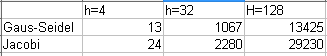
\includegraphics[width=0.7\textwidth]{bilder/convergenz.png}
  \caption{Über zehn Aufrufe gemittelte Anzahl Iterationen in beiden Verfahren für verschiedene Verfeinerungen $h$, bis unser Abbruchkriterium \texttt{true} wurde.}
  \label{fig:Bild1}
\end{figure}

\section{Sequentielle Implementierung}

Die Matrixeinträge werden in dem auf dem Aufgabenblatt zur Verfügung gestellten Pseudocode spaltenweise durchlaufen. Daher haben wir in unserer Implementierung die Matrizen spaltenweise indiziert, um eine möglichst gute Cache-Lokalität zu erzielen. Dies bedeutet, dass wir statt $U$ eigentlich $U^T$ speichern.

Anstatt des Parameters $h$ übergeben wir einen Parameter $size$, der $\left(\frac{1}{h}+1\right)$ entspricht. Dies hat den Vorteil, dass der Nutzer den Grad der Verfeinerung exakt ohne viele Nachkommastellen angeben kann und $U$ eine $size \times size$-Matrix ist.
Um von $size$ auf $h$ zurückzurechnen, gilt:
$$size = \left(\frac{1}{h} + 1\right)$$
$$\Leftrightarrow \frac{1}{h} = size - 1$$
$$\Leftrightarrow h = \frac{1}{size - 1}$$
 
Da sich die Einträge des Vektors $b$ innerhalb der Iterationen nicht ändern, haben wir $b$ vorberechnet.

Den Startvektor haben wir mit zufälligen Gleitkommazahlen gefüllt.

\subsection{Laufzeiten bei verschiedenen Verfeinerungen}
Wir haben die Laufzeiten unser sequentiellen Implementierungen für $h=\frac{1}{2^l}$ mit $l \in \{6, 7, 8, 9, 10\}$ gemessen, da für kleinere Werte von $l$ die Messungen zu stark variierten. Wir haben die Messungen auf \texttt{i82sn02.itec.kit.edu} (Abb.~\ref{fig:seq_sn02}) durchgeführt.

\begin{figure}[h]
\centering
\begin{tabular}{c|c|c|c|c|c}
 & $h=1/64$ & $h=1/128$ & $h=1/256$ & $h=1/512$ & $h=1/1024$ \\ 
\hline
Jacobi & 0.113 s & 1.5 s & 20.7 s & 345 s & 4500 s \\ 
\hline
Gauß-Seidel & 0.113 s & 1.4 s & 14.8 s & 115 s & 545 s
\end{tabular}

\caption{Laufzeiten der sequentiellen Implementierungen des Jacobi- und Gauß-Seidel-Verfahrens für verschiedene Verfeinerungen $h$ auf \texttt{i82sn02.itec.kit.edu}}
\label{fig:seq_sn02}
\end{figure}

\newpage
\subsection{Approximationsfehler}

Wir haben den maximalen absoluten Approximationsfehler in der euklidischen Norm in jedem Iterationsschritt für das Jacobi- und das Gauß-Seidel-Verfahren gemessen. Sei $U^{(*)}$ die analytische Lösung für $U$. Der maximale absolute Approximationsfehler in euklidischer Norm in Iteration $k$ ist definiert als
$$ \max_{(i,j) \in \{1, \ldots, n\}^2} \sqrt{\left({U_{i,j}^{(k)}} - {U_{i,j}^{(*)}}\right)^2}$$

Sei $x_i=i*h$ und $y_j=j*h$ für $i,j = 0, \ldots, n+1$. Wir haben die analytische Lösung mittels der Funktion $u(x_i,y_j) = \begin{cases} 16x_i(1-x_i)y_i(1-y_i) & \text{, falls } 0 < x_i < 1 \text{ und } 0 < y_j < 1 \\ 0 & \text{, sonst} \end{cases}$ berechnet.

Wir haben die Messungen nur für die Verfeinerungen $h \in \left \{\frac{1}{4}, \frac{1}{8}, \frac{1}{16}, \frac{1}{32} \right\}$ durchgeführt, da für kleinere $h$ die Grafiken zu groß werden und man nichts mehr erkennt. Die Grafiken haben wir mit \texttt{gnuplot} erstellt. Beim Vergleich der Grafiken fällt auf, dass der maximale Approximationsfehler beim Gauß-Seidel-Verfahren schneller sinkt als beim Jacobi-Verfahren. Außerdem kann es in beiden Verfahren zu einer geringfügigen Verschlechterung des maximalen Approximationsfehlers in den ersten Iterationen kommen.

\begin{center}
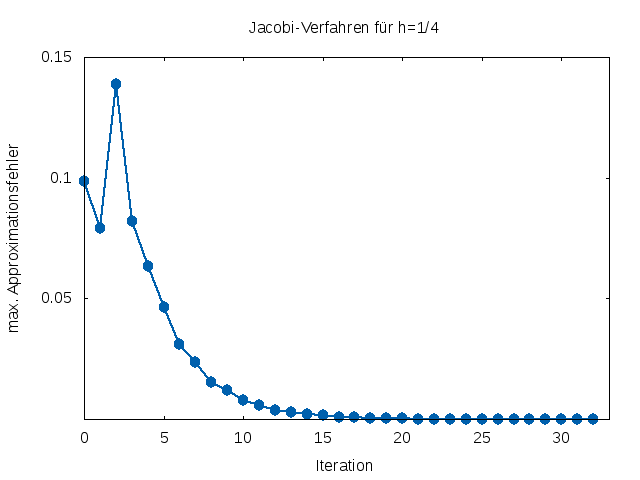
\includegraphics[scale=0.8]{bilder/fehler_jacobi_1_4.png}
\end{center}

\begin{center}
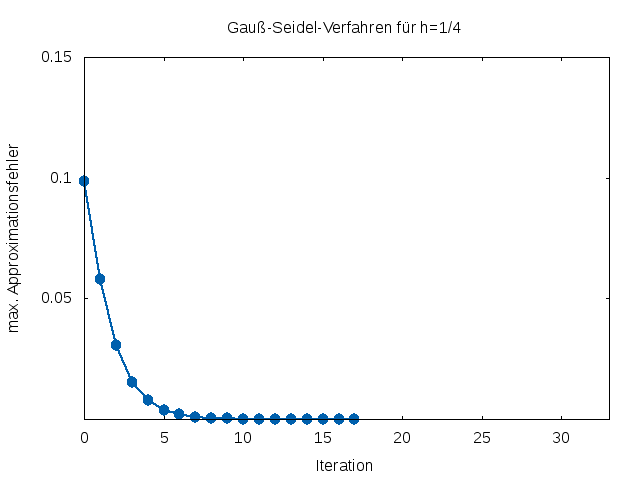
\includegraphics[scale=0.8]{bilder/fehler_gs_1_4.png}
\end{center}

\begin{center}
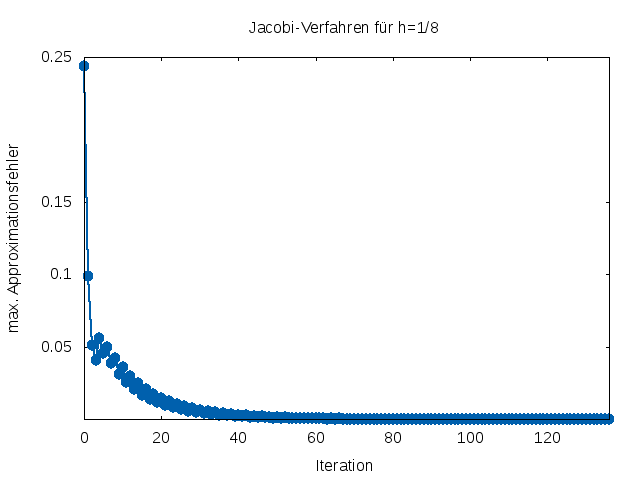
\includegraphics[scale=0.8]{bilder/fehler_jacobi_1_8.png}
\end{center}

\begin{center}
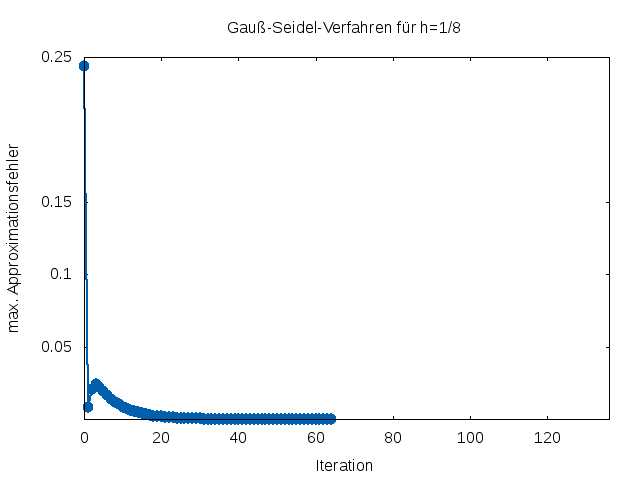
\includegraphics[scale=0.8]{bilder/fehler_gs_1_8.png}
\end{center}

\begin{center}
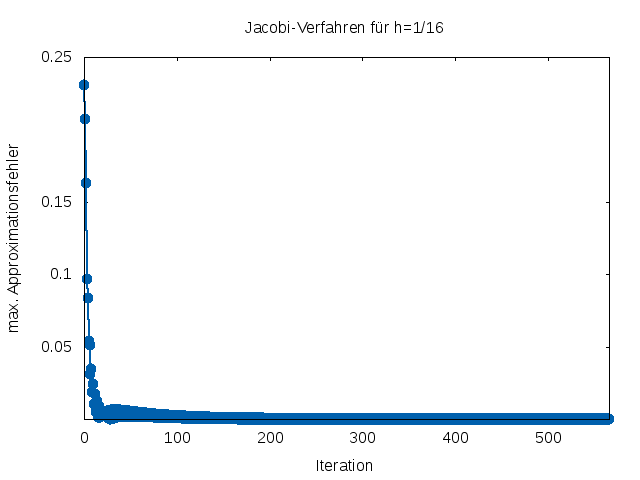
\includegraphics[scale=0.8]{bilder/fehler_jacobi_1_16.png}
\end{center}

\begin{center}
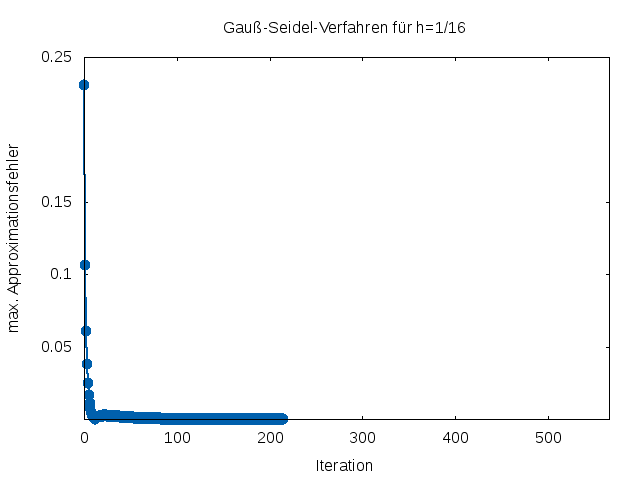
\includegraphics[scale=0.8]{bilder/fehler_gs_1_16.png}
\end{center}

\begin{center}
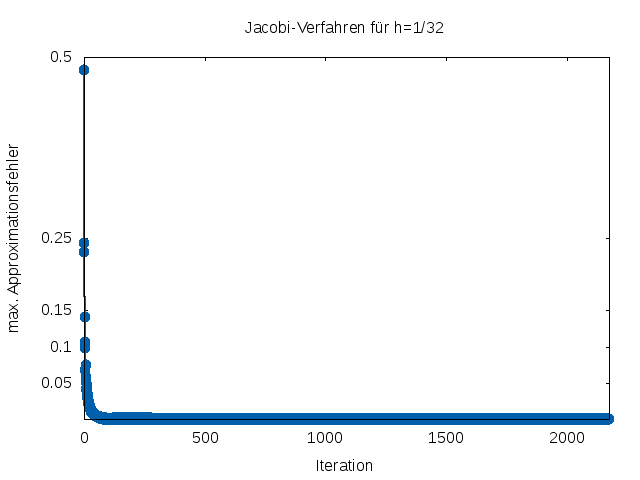
\includegraphics[scale=0.8]{bilder/fehler_jacobi_1_32.png}
\end{center}

\begin{center}
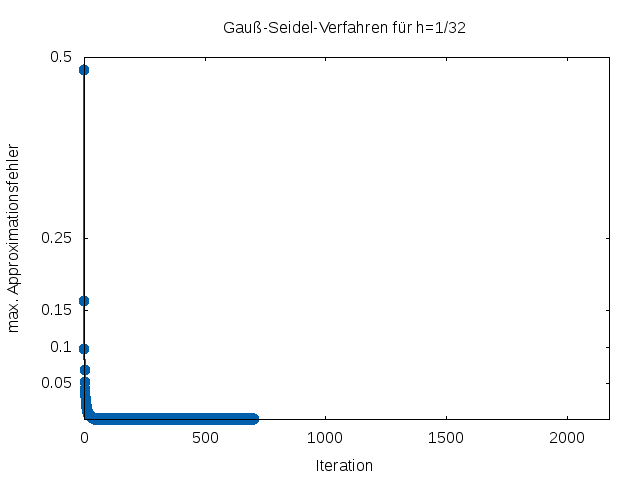
\includegraphics[scale=0.8]{bilder/fehler_gs_1_32.png}
\end{center}

\section{Parallelisierung}

\subsection{Jacobi-Verfahren} \label{parallel:jacobi}
Da innerhalb der Iterationsschritte des Jacobi-Verfahrens keinerlei Datenabhängigkeiten bei der Berechnung der Matrixeinträge bestehen, haben wir mittels OpenMP (\texttt{\#pragma omp parallel for}) die äußere Schleife parallelisiert.

Zudem haben wir eine weitere Version des Jacobi-Verfahrens implementiert, in der wir zusätzlich zur Parallelisierung der \texttt{for}-Schleife auch den Code innerhalb der \texttt{for}-Schleife mit SSE vektorisiert haben.

Hierbei haben wir folgenden Speedup bei verschiedenen Problemgrößen $h$ und sowie verschiedenen Prozessorzahlen $p$ gemessen: \ref{ergebnisse}

\subsection{Gauß-Seidel-Verfahren}

Innerhalb der Iterationsschritte des Gauß-Seidel-Verfahrens bestehen Datenabhängigkeiten, da die Berechnung der Matrixeinträge in einer Iteration von den vorher berechneten Einträgen der selben Iteration abhängt. Das Gauß-Seidel-Verfahren ist daher inhärent sequentiell. Daher ist eine Parallelisierung des Gauß-Seidel-Verfahrens mit mehr Aufwand verbunden als beim ``embarassingly parallel'' Jacobi-Verfahren.

Wir haben sowohl den naiven, falschen Parallelisierungsansatz als auch zwei verschiedene funktionierende Parallelisierungsansätze implementiert.

\subsubsection{Naiver Parallelisierungsansatz}\label{gs:naiv}
Der naive Parallelisierungsansatz ist, wie in Abschnitt~\ref{parallel:jacobi} die äußerste Schleife mittels \texttt{\#pragma omp parallel for} zu parallelisieren. Da eine parallele Ausführung der Schleifeniterationen mittels OpenMP nicht die Iterationsreihenfolge garantiert, kann es hierbei zu Wettlaufsituationen (``Race Conditions'') kommen.

Der im Praktikum vorgestellte Intel Thread Checker erkennt die auftretende Wettlaufsituation nicht.

\begin{figure}[h] 
  \centering
     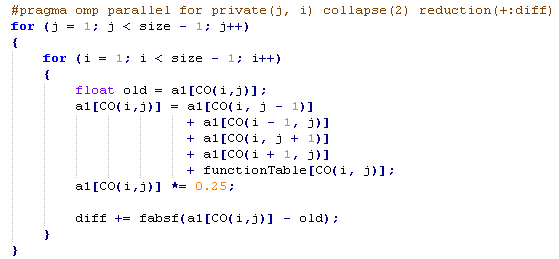
\includegraphics[width=1.0\textwidth]{bilder/race.png}
  \caption{Naive Parallelisierung des Gauß-Seidel-Verfahrens. Hierbei kann es zu Wettlaufsituationen kommen, da nicht garantiert ist, in welcher Reihenfolge beispielsweise auf den Eintrag  \texttt{a1[CO(i,j+1)]} zugegriffen wird.}
\end{figure}

\subsubsection{Erweiterter Parallelisierungsansatz: Rot-Schwarz}

Bei der Rot-Schwarz-Parallelisierung des Gauß-Seidel-Verfahrens wird ausgenutzt, dass jeder Matrixeintrag nur von seinem linken, rechten, oberen und unteren direkten Nachbarn abhängt. Wir färben also die Matrixeinträge in rote und schwarze Felder ein, wobei die Datenabhängigkeiten nur zwischen Einträgen unterschiedlicher Farbe bestehen. Hierbei ergibt sich ein Schachbrettmuster, wie in Abbildung~\ref{fig:matrix} gezeigt.

\begin{figure}[h!]
\centering
$$U = 
\begin{tabular}{cccccc}
  \cellcolor{rose} & \cellcolor[gray]{0.7} & \cellcolor{rose} & \cellcolor[gray]{0.7} & \cellcolor{rose} & \cellcolor[gray]{0.7}\\
 \cellcolor[gray]{0.7} & \cellcolor{red} & \cellcolor[gray]{0.45} & \cellcolor{red} & \cellcolor[gray]{0.45} & \cellcolor{rose}\\
  \cellcolor{rose} & \cellcolor[gray]{0.45} & \cellcolor{red} & \cellcolor[gray]{0.45} & \cellcolor{red} & \cellcolor[gray]{0.7}\\
 \cellcolor[gray]{0.7} & \cellcolor{red} & \cellcolor[gray]{0.45} & \cellcolor{red} & \cellcolor[gray]{0.45} & \cellcolor{rose} \\
 \cellcolor{rose} & \cellcolor[gray]{0.45} & \cellcolor{red} & \cellcolor[gray]{0.45} & \cellcolor{red} & \cellcolor[gray]{0.7}\\
 \cellcolor[gray]{0.7} & \cellcolor{rose} & \cellcolor[gray]{0.7} & \cellcolor{rose} & \cellcolor[gray]{0.7} & \cellcolor{rose}\\
\end{tabular}
$$
\caption{Aufteilung der Lösungsmatrix $U$ in rote und schwarze Zellen, sodass zwischen Zellen gleicher Farbe keine Datenabhängigkeiten bestehen. Die Randzellen, deren Einträge per Annahme immer den Wert $0$ enthalten, sind in blasseren Farben markiert.}
\label{fig:matrix}
\end{figure}

Da die Matrixeinträge gleicher Farbe nicht voneinander abhängen, können wir diese parallel berechnen. Dies führt zu dem Ansatz, zuerst alle roten Einträge und danach alle schwarzen Einträge jeweils parallel zu berechnen.

Hierbei ist zu beachten, dass die einzelnen Iterationen des sequentiellen Gauß-Seidel-Verfahrens und dessen Rot-Schwarz-Parallelisierung nicht genau dasselbe Ergebnis liefern. Dies liegt darin begründet, dass durch die Rot-Schwarz-Aufteilung eine Umordnung der Matrixeinträge geschieht.

Um die Indexberechnung zu vereinfachen und die Cachelokalität zu verbessern, haben wir die roten und die schwarzen Einträge jeweils in eigenen, neuen Matrizen gespeichert. Dadurch liegen Einträge gleicher Farbe zusammenhängend im Speicher. Dies hat es uns auch ermöglicht, unsere Implementierung mittels SSE-Vektorinstruktionen zu beschleunigen. Die Vektorisierung mittels SIMD-Instruktionen haben wir explizit implementiert. Zwar ist mit OpenMP 4.0 eine Vektorisierung von Code auch mittels \texttt{\#pragma omp simd} möglich, aber unser händisch vektorisierter Code war schneller als der von OpenMP generierte.

Bei den Indexberechnungen haben wir zwischen $size \times size$-Matrizen gerader und ungerader $size$ unterschieden.

\paragraph{Berechnung der Nachbarindizes für gerade Werte von $size$}~\\
Für rote $U_{i,j}$ gilt: Der zugehörige Index in der Matrix für die roten Einträge ist $idx = \lfloor\frac{i+j*size}{2}\rfloor$. Der linke Nachbar ist an Stelle $idx - \frac{size}{2}$ in der Schwarz-Matrix. Der obere Nachbar ist an Stelle $idx - (1-(j \mod 2))$ in der Schwarz-Matrix. Der rechte Nachbar ist an Stelle $idx + \frac{size}{2}$ in der Schwarz-Matrix. Der untere Nachbar ist an Stelle $idx + (j \mod 2)$ in der Schwarz-Matrix.



Für schwarze $U_{i,j}$ gilt: Der zugehörige Index in der Matrix für die schwarzen Einträge ist $idx = \lfloor\frac{i+j*size}{2}\rfloor$. Der linke Nachbar ist an Stelle $idx - \frac{size}{2}$ in der Rot-Matrix. Der obere Nachbar ist an Stelle $idx - (j \mod 2)$ in der Rot-Matrix. Der rechte Nachbar ist an Stelle $idx + \frac{size}{2}$ in der Rot-Matrix. Der untere Nachbar ist an Stelle $idx + (1- (j \mod 2))$ in der Rot-Matrix.

Abbildung~\ref{fig:matrix:even} zeigt die Berechnung der Nachbarindizes am Beispiel $size=6$.

\begin{figure}[h!]
\centering
$$U = 
\begin{tabular}{cccccc}
  \cellcolor{rose}0 & \cellcolor[gray]{0.7}3 & \cellcolor{rose}6 & \cellcolor[gray]{0.7}9 & \cellcolor{rose}12 & \cellcolor[gray]{0.7}15\\
  
 \cellcolor[gray]{0.7}0 & \cellcolor{red}3 & \cellcolor[gray]{0.45}6 & \cellcolor{red}9 & \cellcolor[gray]{0.45}12 & \cellcolor{rose}15\\
 
  \cellcolor{rose}1 & \cellcolor[gray]{0.45}4 & \cellcolor{red}7 & \cellcolor[gray]{0.45}10 & \cellcolor{red}13 & \cellcolor[gray]{0.7}16\\
  
 \cellcolor[gray]{0.7}1 & \cellcolor{red}4 & \cellcolor[gray]{0.45}7 & \cellcolor{red}10 & \cellcolor[gray]{0.45}13 & \cellcolor{rose}16 \\
 
 \cellcolor{rose}2 & \cellcolor[gray]{0.45}5 & \cellcolor{red}8 & \cellcolor[gray]{0.45}11 & \cellcolor{red}14 & \cellcolor[gray]{0.7}17\\
 
 \cellcolor[gray]{0.7}2 & \cellcolor{rose}5 & \cellcolor[gray]{0.7}8 & \cellcolor{rose}11 & \cellcolor[gray]{0.7}14 & \cellcolor{rose}17\\
\end{tabular} \quad
$$

$\textcolor{red}{\leftarrow: idx - \frac{size}{2}} \quad$
$\textcolor{red}{\rightarrow: idx + \frac{size}{2}} \quad$
$\textcolor{red}{\uparrow: idx - (1-(j \mod 2))} \quad$
$\textcolor{red}{\downarrow: idx + (j \mod 2)} \quad$

$\textcolor{black}{\leftarrow: idx - \frac{size}{2}} \quad$
$\textcolor{black}{\rightarrow: idx + \frac{size}{2}} \quad$
$\textcolor{black}{\uparrow: idx - (j \mod 2)} \quad$
$\textcolor{black}{\downarrow: idx + (1- (j \mod 2))} \quad$

\caption{Berechnung der Nachbarindizes für gerade Werte von $size$ am Beispiel $size=6$}
\label{fig:matrix:even}
\end{figure}

\paragraph{Berechnung der Nachbarindizes für ungerade Werte von $size$}~\\
Für rote $U_{i,j}$ gilt: Der zugehörige Index in der Matrix für die roten Einträge ist $idx = \lfloor\frac{i+j*size}{2}\rfloor$. Der linke Nachbar ist an Stelle $idx - \lceil\frac{size}{2}\rceil$ in der Schwarz-Matrix. Der obere Nachbar ist an Stelle $idx - 1$ in der Schwarz-Matrix. Der rechte Nachbar ist an Stelle $idx + \lfloor\frac{size}{2}\rfloor$ in der Schwarz-Matrix. Der untere Nachbar ist an Stelle $idx$ in der Schwarz-Matrix.



Für schwarze $U_{i,j}$ gilt: Der zugehörige Index in der Matrix für die schwarzen Einträge ist $idx = \lfloor\frac{i+j*size}{2}\rfloor$. Der linke Nachbar ist an Stelle $idx - \lfloor\frac{size}{2}\rfloor$ in der Rot-Matrix. Der obere Nachbar ist an Stelle $idx$ in der Rot-Matrix. Der rechte Nachbar ist an Stelle $idx + \lceil\frac{size}{2}\rceil$ in der Rot-Matrix. Der untere Nachbar ist an Stelle $idx + 1$ in der Rot-Matrix.

Abbildung~\ref{fig:matrix:odd} zeigt die Berechnung der Nachbarindizes am Beispiel $size=7$.

\begin{figure}[h!]
\centering
$$U = 
\begin{tabular}{ccccccc}
  \cellcolor{rose}0 & \cellcolor[gray]{0.7}3 & \cellcolor{rose}7 & \cellcolor[gray]{0.7}10 & \cellcolor{rose}14 & \cellcolor[gray]{0.7}17 & \cellcolor{rose}21 \\
  
 \cellcolor[gray]{0.7}0 & \cellcolor{red}4 & \cellcolor[gray]{0.45}7 & \cellcolor{red}11 & \cellcolor[gray]{0.45}14 & \cellcolor{red}18 & \cellcolor[gray]{0.7}21\\
 
  \cellcolor{rose}1 & \cellcolor[gray]{0.45}4 & \cellcolor{red}8 & \cellcolor[gray]{0.45}11 & \cellcolor{red}15 & \cellcolor[gray]{0.45}18 & \cellcolor{rose}22\\
  
 \cellcolor[gray]{0.7}1 & \cellcolor{red}5 & \cellcolor[gray]{0.45}8 & \cellcolor{red}12 & \cellcolor[gray]{0.45}15 & \cellcolor{red}19 & \cellcolor[gray]{0.7}22\\
 
 \cellcolor{rose}2 & \cellcolor[gray]{0.45}5 & \cellcolor{red}9 & \cellcolor[gray]{0.45}12 & \cellcolor{red}16 & \cellcolor[gray]{0.45}19 & \cellcolor{rose}23\\
 
 \cellcolor[gray]{0.7}2 & \cellcolor{red}6 & \cellcolor[gray]{0.45}9 & \cellcolor{red}13 & \cellcolor[gray]{0.45}16 & \cellcolor{red}20 & \cellcolor[gray]{0.7}23\\
 
 \cellcolor{rose}3 & \cellcolor[gray]{0.7}6 & \cellcolor{rose}10 & \cellcolor[gray]{0.7}13 & \cellcolor{rose}17 & \cellcolor[gray]{0.7}20 & \cellcolor{rose}24 \\
\end{tabular} \quad
$$


$\textcolor{red}{\leftarrow: idx - \lceil\frac{size}{2}\rceil} \quad$
$\textcolor{red}{\rightarrow: idx + \lfloor\frac{size}{2}\rfloor} \quad$
$\textcolor{red}{\uparrow: idx - 1} \quad$
$\textcolor{red}{\downarrow: idx} \quad$

$\textcolor{black}{\leftarrow: idx - \lfloor\frac{size}{2}\rfloor} \quad$
$\textcolor{black}{\rightarrow: idx + \lceil\frac{size}{2}\rceil} \quad$
$\textcolor{black}{\uparrow: idx} \quad$
$\textcolor{black}{\downarrow: idx + 1} \quad$

\caption{Berechnung der Nachbarindizes für ungerade Werte von $size$ am Beispiel $size=7$}
\label{fig:matrix:odd}
\end{figure}

\newpage

\paragraph{Messung von Speedup und Effizienz unter verschiedenen Verfeinerungen, Skalierbarkeit} 
TODO

\subsubsection{Erweiterter Parallelisierungsansatz: Wavefront}
Beim Wavefront Algorithmus wird anstatt über die Spalten oder Zeilen zu iterieren über die Antidiagonalen iteriert. Das hat den Vorteil, dass die Daten nicht voneinander abhängig sind und das selbe herauskommt, wie beim eigentlichen Gauß-Seidel Verfahren in serieller Form.

Vermutlicher Grund wieso unsere Wavefront-Implementierung langsamer als sequentielles Gauß-Seidel: Die Indexberechnung ist sehr aufwändig. Wir berechnen  die Indizes in jeder Iteration neu, anstatt sie einmalig vorzuberechnen und in einer ``Indextabelle'' zu speichern. Außerdem richtet sich die Parallelität nach der Anzahl der Antidiagonalelemente. D.h. es lohnt sich erst bei großen Antidiagonalen.

Bei der Wavefront Cache Lösung wurden die Matrix zuerst in ein anderes Array kopiert, in dem die Antidiagonalen in den Zeilen stehen. Dadurch haben wir uns erhofft, dass es zu einer höheren Cache Hitrate kommt. \\
In beiden Wavefront Lösungen hätte man sicher noch einiges optimieren können(z.B. CUDA für große Antidiagonalen), jedoch erschien uns Rot-Schwarz so viel schneller, dass es sich nicht lohnen würde.

\paragraph{Berechnung der Indizes}
Für die Implementierung wurden drei Schleifen verwendet. Die äußere Schleife ist zwischen den Schritten des Gauß-Seidel Verfahrens, die mittlere geht über die Antidiagonalen und die innere über die Elemente der Antidiagonalen. \\
In der mittleren Schleife werden die Variablen für die aktuelle Anzahl an Elementen gesteuert sowie eine Variable die angibt in welchem Durchlauf man nach der Antidiagonalen ist(border). Diese dient dazu anzugeben, wie viele Elemente man am Rand weglassen kann, weil sie nicht mehr in der Matrix sind.\\
Bei der Wavefront Cache Lösung muss man bei jeder Indexberechnung die Eingangspermutation, welche die Antidiagonalen den Zeilen des Arrays zuweist umkehren um die Indizes zu berechnen. Hierbei verwenden wir die Hilfsvariablen \texttt{hack} und \texttt{hack2}. Diese werden benutzt um die Elemente um das zu berechnende Element zu adressieren. Die Variable \texttt{hack} wird 1 Durchgang vor der Antidiagonalen zu 1, weil sich ab hier die Abhängigkeit der Elemente um 1 verschiebt. Das selbe gilt für \texttt{hack2} ab der mittleren Antidiagonalen. \\
Da der Ansatz nicht so viel schneller wurde, dass man Rot-Schwarz hätte schlagen können, wurde der Algorithmus nicht platzeffizient implementiert und die Matrixgröße ist größer als bei den anderen Algorithmen. Es wäre jedoch auch möglich gewesen dieselbe Matrixgröße zu verwenden.

\begin{figure}[h] 
  \centering
     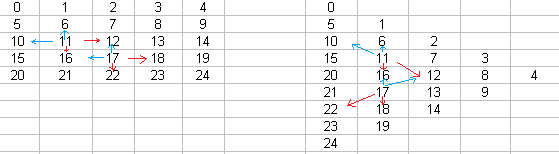
\includegraphics[width=1\textwidth]{bilder/hack.png}
  \caption{Veranschaulichung der Permutation, welche verwendet wird sowie der Verschiebung der Indizes anhand eines Beispiels. Die Variable \texttt{hack} ist dabei blau und \texttt{hack2} rot.}
  \label{fig:Bild6}
\end{figure}

\section{Methodenwahl}
Es empfiehlt sich das Gauß-Seidel-Verfahren zu nutzen, weil es im allgemeinen schneller konvergiert als das Jacobi-Verfahren. Bis zu einer Matrixgröße von $size \times size$ mit $size = 31$ (was $h=\frac{1}{30}$ entspricht) lohnt sich das Parallelisieren nicht. Bei größeren Matrizen (also $h < \frac{1}{30}$) ist die Rot-Schwarz SSE Implementierung des Gauß-Seidel Verfahrens am schnellsten.

TODO: Laufzeitmessungen

\end{document}
